\chapter{Online reprocessing modeling approach}
\section{Fuel salt reprocessing overview} \label{sec:reproc-plant}
Removing specific chemical elements from a molten salt is a complicated 
task that requires intelligent design (e.g., chemical separations equipment 
design, fuel salt flows to equipment). This section contains a brief overview 
of a generic \gls{MSR} fuel salt reprocessing system. Modeling such systems is 
the focus of the current dissertation.

\subsection{Gas separation system} \label{sec:gas-separ}
Gaseous fission products (e.g., Kr, Xe) must be removed from the fuel salt 
to avoid reactor poisoning, especially during startup and power maneuvering. 
This is particularly true for $^{135}$Xe, with its extensive neutron capture 
cross section ($\approx10^6\dots10^7$ b in a thermal energy range). $^{135}$Xe 
is produced directly from fission in about 0.3\% of $^{235}$U fissions 
($\gamma_{_{^{135}Xe}}$), but an even larger fraction of $^{135}$Xe is 
produced by the decay of $^{135}$I and $^{135}$Te (table~\ref{tab:xe_gain}). 
$^{135}$I and $^{135}$Te yields from fission are 
$\gamma_{_{^{135}I}}\!=3.6$\% and $\gamma_{_{^{135}Te}}\!=2.5$\%, 
respectively. Thus, the total $^{135}$Xe production from fission is about 
6.4\% of fissions (of $^{235}$U), most of this is from $^{135}$I and 
$^{135}$Te decay. Noble gases (e.g., tritium, xenon, and krypton) can be 
removed from the fuel salt as follows:
\begin{enumerate}[label=(\alph*)]
	\item a bubble generator injects helium bubbles in the salt stream;
	\item noble gases migrate promptly to the helium bubbles because 
	of their extreme insolubility in the salt 
	\cite{robertson_conceptual_1971};
	\item and a gas separator discharges the fission-product-rich bubbles from 
	the salt to the off-gas system.
\end{enumerate}
%%%%%%%%%%%%%%%%%%%%%%%%%%%%%%%%%%%%%%%%%%%%%%%%%%%%%%%%%%%%%
\begin{table}[ht!]
	\caption{$^{135}$Xe production sources and principal rate constants 
		involved
		(reproduced from Kedl \emph{et al.} \cite{kedl_development_1967}).}
	\centering
	\begin{tabularx}{\textwidth}{b  b}
		\hline \textbf{$^{135}$Xe gain mechanism} & \textbf{Principal rate 
			parameters involved}  	\\ [5pt] \hline 
		Direct from fission & $\Sigma_f \gamma_{_{^{135}Xe}}\phi$ (for 
		$^{235}$U fission) \\
		yield $\gamma_{_{^{135}Xe}}\!\!\!=0.003$ & \\ [5pt] \hline 
		$^{135}$I decay     & $\Sigma_f \gamma_{_{^{135}I}}\phi$ (for 
		$^{235}$U fission) \\
		yield $\gamma_{_{^{135}Xe}}\!\!\!=0.036$, it decays to $^{135}$Xe with 
		$\tau_{1/2}=6.68$ h & 			                    \\	[5pt]	\hline 
		$^{135}$Te decay    & $\Sigma_f \gamma_{_{^{135}Te}}\phi$ (for 
		$^{235}$U 		fission) \\
		yield $\gamma_{_{^{135}Xe}}\!\!\!=0.025$, 
		it decays to $^{135}$I with $\tau_{1/2}=19$ s 
		& 			                    \\ [5pt]	\hline
	\end{tabularx}
	\label{tab:xe_gain}
\end{table}
%%%%%%%%%%%%%%%%%%%%%%%%%%%%%%%%%%%%%%%%%%%%%%%%%%%%%%%%%%%%%%%%%%%
Diagram~\ref{fig:xe_diagram} shows the key pathways for xenon production, 
accumulation, and removal in a typical \gls{MSR}.  
Figure~\ref{fig:gas_removal_system} shows the conceptual design of the  
\gls{MSBR} gas separation system. Helium bubbles of a specific size are 
introduced in a salt stream via the primary pump bowl. These bubbles absorb 
noble gases before being separated from the salt by a gas separator. 
\gls{ORNL} suggested that the \gls{MSBR} off-gas system would inject 
$d=0.508$mm helium bubbles in the pump bowl, redirect 10\% of the fuel salt 
flow through a bubble separator to remove the bubbles, and then return the 
flow into the pump suction. Robertson \emph{et al.} reported that the helium 
bubble size was approximately 25\% of the throat width (blue circle on 
figure~\ref{fig:bubble_separator}) and was independent of the gas flow rate 
\cite{robertson_conceptual_1971}. Consequently, it is possible to regulate the 
helium bubble size by changing the throat width in the bubble generator.
\begin{figure}[htp!] % replace 't' with 'b' to 
	\centering
	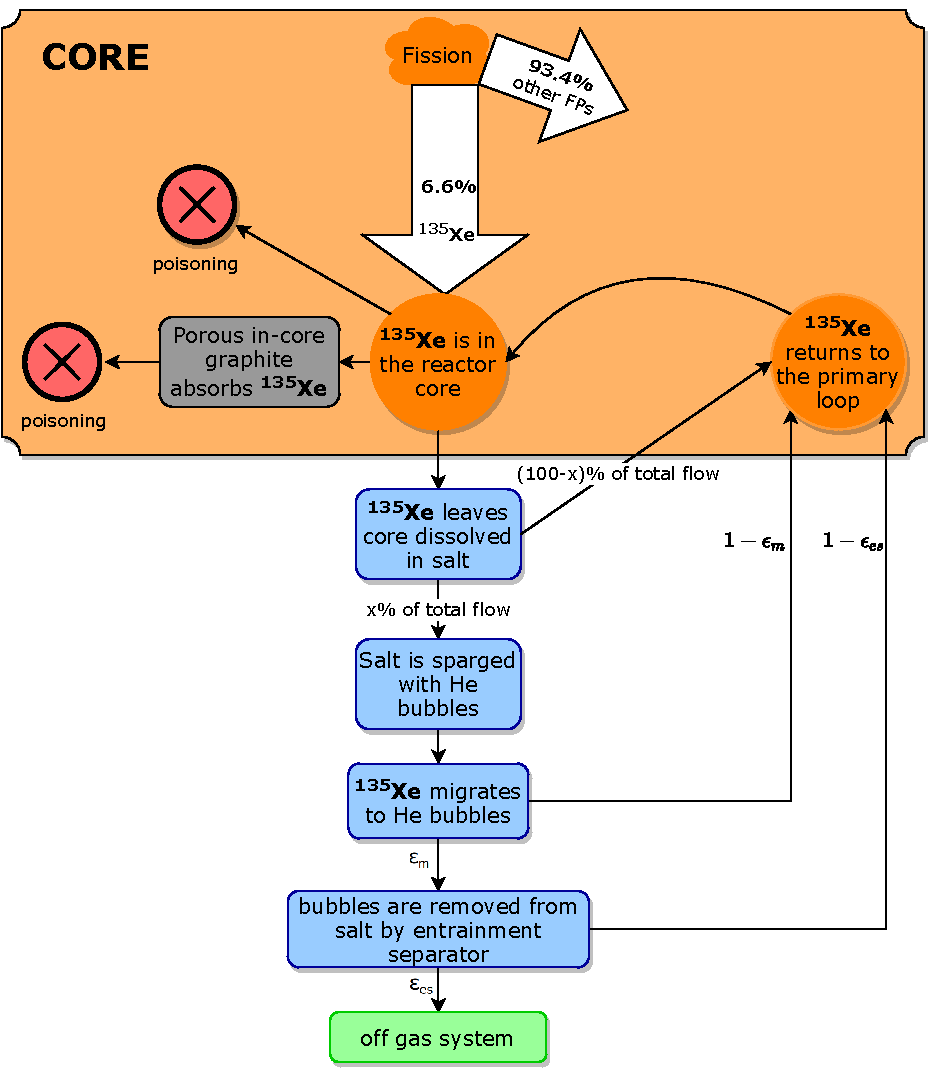
\includegraphics[width=1.01\textwidth]{ch2/xe_diagram.pdf}
	\caption{Schematic of $^{135}$Xe circulation in a generic \gls{MSR}. $x$ 
	is the fraction of fuel salt flow from the pump discharge redirected to 
	the gas separation system, while $\epsilon_m$ and $\epsilon_{es}$ are the 
	efficiencies of migration (of $^{135}$Xe to the helium bubbles in the 
	sparger) and separation (of gas in the entrainment separator), 
	respectively. The orange color represents the fuel salt in the primary 
	loop, the blue color represents the gas separation system, and the gray 
	color is the moderator in the core. Fission yields assume $^{235}$U 
	fission 	only.}
	\label{fig:xe_diagram}
\end{figure}
\begin{figure}[htp!] % replace 't' with 'b' to 
	\centering
	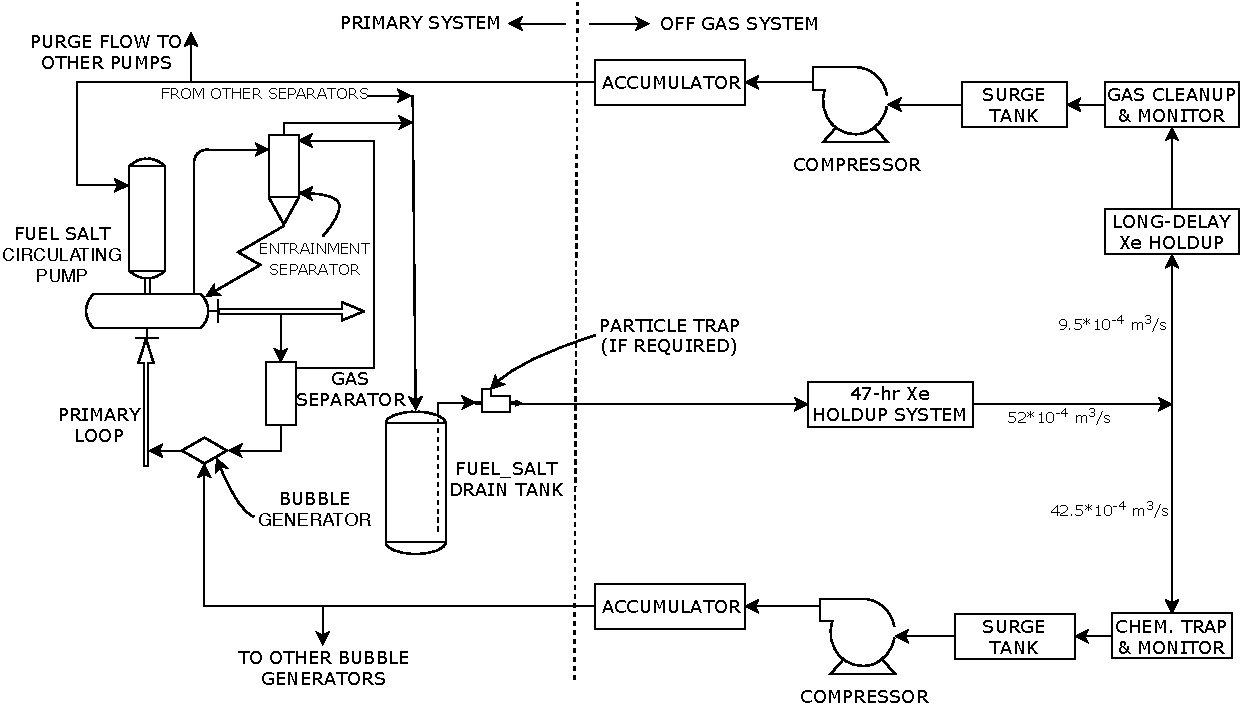
\includegraphics[width=1.02\textwidth]{ch2/gas_separation.pdf}
	\caption{Schematic flow diagram of the \gls{MSBR} gas separation system 
		(figure reproduced from Robertson \emph{et al.} 
		\cite{robertson_conceptual_1971}).}
	\label{fig:gas_removal_system}
\end{figure}
\begin{figure}[htp!] % replace 't' with 'b' to 
	\centering
	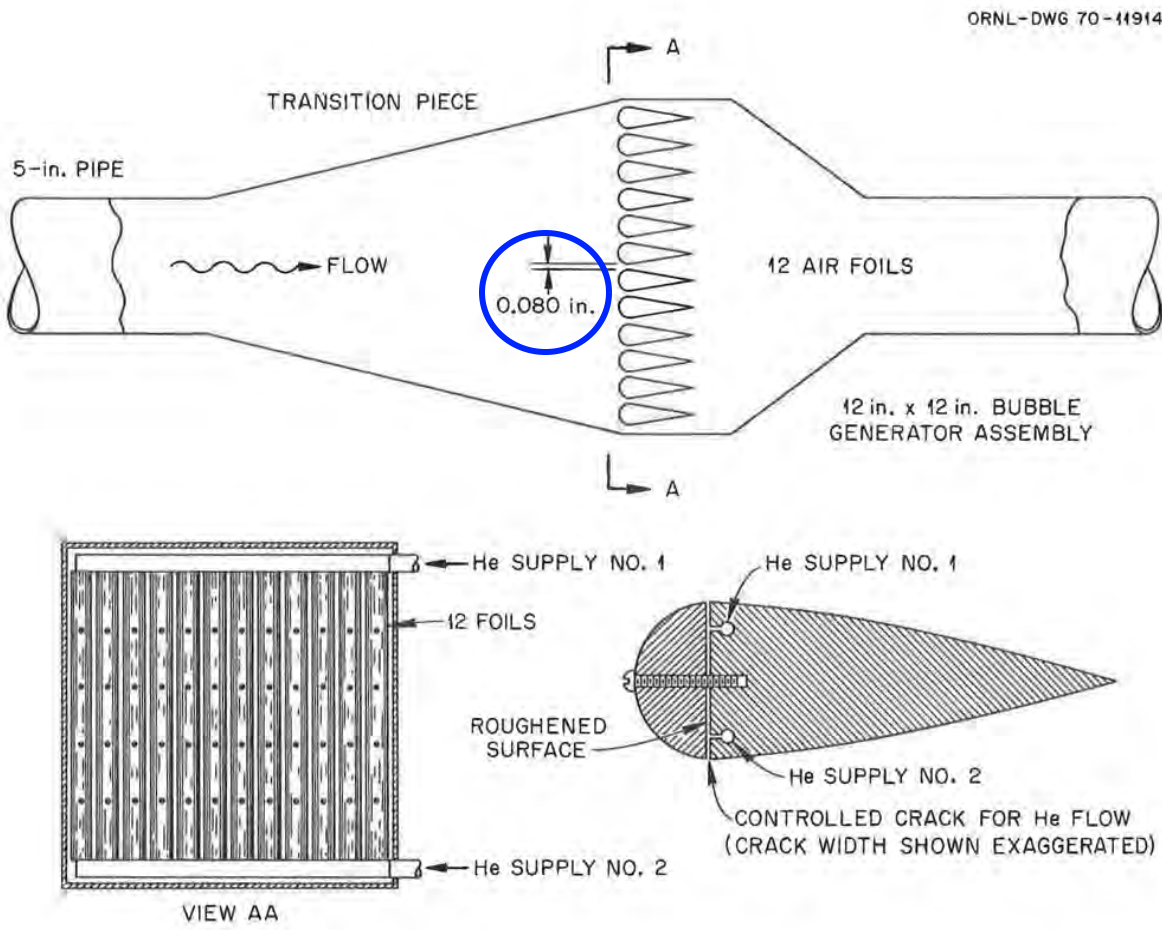
\includegraphics[width=0.77\textwidth]{ch2/msbr_bubble_generator.png}
	\caption{Preliminary concept of \gls{MSBR} bubble generator (figure 
		reproduced from Robertson \emph{et al.} 
		\cite{robertson_conceptual_1971}). 
		The blue circle shows throat width, which determines bubble size.}
	\vspace{-0.25in}
	\label{fig:bubble_separator}
\end{figure}
\begin{table}[b]
	\caption{$^{135}$Xe loss terms and principal rate constants involved
		(reproduced from Kedl \emph{et al.} \cite{kedl_development_1967}).}
	\centering
	\begin{tabularx}{\textwidth}{b b}
		\hline \textbf{$^{135}$Xe loss mechanism}      & \textbf{Principal 
			rate 
			parameters involved}  	\\
		\hline Decay of dissolved $^{135}$Xe ($\tau_{1/2}=9.1$ h)  & Decay 
		constant	($\lambda$)		\\
		\hline $^{135}$Xe burnup              &  Neutron flux 
		($\phi$)		 					\\
		dissolved xenon-135 burnup as it passes through the core  
		& 			            \\		\hline $^{135}$Xe migrated to 
		helium bubbles & Removal efficiency 
		($\epsilon_m$)		\\
		\hline $^{135}$Xe transferred into circulating He bubbles; this xenon 
		will eventually be burnup, decay, or stripped via bubble separator & 
		Mass transfer coefficient ($h$), decay constant ($\lambda$), 
		neutron flux ($\phi$), bubble removal efficiency 
		($\epsilon_{es}$)		\\
		\hline 
	\end{tabularx}
	\label{tab:xe_loss}
\end{table}

To realistically model the gas separation system, we need a mathematical model 
that describes noble gas extraction efficiency during reactor operation. 
Particularly, a model of xenon extraction efficiency as a function of sparger 
design parameters is needed to accurately model the $^{135}$Xe removal in a 
fuel salt depletion simulation. The gain and loss terms for $^{135}$Xe 
dissolved in the fuel salt are listed in Tables~\ref{tab:xe_gain} and 
\ref{tab:xe_loss}. The removal efficiency for the xenon in the pump bowl was 
measured during \gls{MSRE} operation. However, the the technical report 
ORNL-4069 by Kedl-Houtzeel only stated its range (from 50 to 100\%) and 
concluded, ``It is probably a complex parameter like the circulating-void 
fraction and depends on many reactor operational variables.'' 
\cite{kedl_development_1967}. $^{135}$Xe burnup and decay rates are well 
known. 

Peebles \emph{et al.} in ORNL-TM-2245 has reported xenon removal efficiency 
($\epsilon_{Xe}$) in a gas separation system as a function of many parameters 
\cite{peebles_removal_1968}:
\begin{align}\label{eq:gas_eff}
& \qquad\qquad \epsilon_{Xe} = \frac{1-e^{-\beta}}{1+\alpha}
\intertext{where}
\alpha &= \frac{RTQ_{salt}}{HQ_{He}} \\
\beta &= \frac{K_L a A_C L (1+\alpha)}{Q_{salt}} \\
R &= \mbox{universal gas constant} \nonumber \\
T &= \mbox{salt temperature} \nonumber \\
Q_{salt}&= \mbox{volumetric salt flow rate} \nonumber \\
Q_{He}&= \mbox{volumetric helium flow rate} \nonumber \\
H &= \mbox{Henry's law constant for solute gas} \nonumber \\
a &= \mbox{gas-liquid interfacial area} \nonumber \\
A_C &= \mbox{contactor cross section} \nonumber \\
L &= \mbox{contactor length} \nonumber \\
K_L &= \mbox{liquid phase mass transfer coefficient.} \nonumber
\end{align}
Most of the input parameters for that correlation are obvious and easy to 
obtain from the system component design. The mass transfer coefficient for 
transferring xenon into helium bubbles ($K_L$) can be estimated  
experimentally, but published information is currently insufficient 
to inform an accurate mathematical model appropriate for \gls{CFD}. Thus, 
Peebles \emph{et al.} reported the mass transfer coefficient correlation for 
the \gls{MSBR} salt (LiF-BeF$_2$-ThF$_4$-UF$_4$) but for a limited case. While 
it is out of the scope of this work to accurately estimate mass transfer 
coefficient, this work seeks to provide a tool which would allow the user to 
specify any mathematical model for a separation efficiency.

Equation~\ref{eq:gas_eff} would apply to other noble gases (e.g., Kr, Ar), but 
Henry's law constant ($H$) and the mass transfer coefficient ($K_L$) would 
be different. Current effort at the University of Illinois at 
Urbana-Champaign, namely, ``Enabling Load Following Capability in the 
Transatomic Power \gls{MSR}," \cite{huff_enabling_2018} has a goal to 
determine mass transfer coefficients for various gaseous fission products (Ar, 
Kr, Xe) using experiments, enabling \gls{CFD} and multi-physics simulations of 
such reactors. As a result, the obtained mathematical model for gas removal 
efficiency might be employed to inform a realistic physics-based fuel 
reprocessing model in SaltProc.


\subsection{Insoluble fission products filtering}
The decay chain of approximately 40\% of fission products has gaseous elements 
in it. Some of the non-gaseous \glspl{FP} produced in the \gls{MSR} core 
(e.g., 
noble and semi-noble metals) have very low solubility in the molten salt. Some 
fraction of noble and semi-noble solid fission products plate out onto the 
internal surfaces of the primary loop equipment, complicating their removal 
\cite{briggs_molten-salt_1964}. The remains noble and semi-noble metals can be 
removed along with corrosion products using a mechanical filtration system, 
which ``consists largely of a high surface area mechanical filter, likely a 
nickel mesh, to promote deposition of suspended, undissolved fission and 
corrosion products,'' stated Holcomb \emph{et al.} 
\cite{holcomb_instrumentation_2018}. The filter is manufactured from porous 
metal and located on a recirculating side stream of the side. The filter has 
limited capacity, needs periodic replacement, and the dose rate on the used 
filter is very high due to the undissolved fission products and residual fuel 
salt remaining on the filter \cite{mcfarlane_review_2019-1}. Differential 
pressure measurements before and after filters are required to determine when 
the filters are full. 

The historic \gls{MSRE} program provided basic information on the design and 
performance of the large mechanical filter. 
Figure~\ref{fig:large_filter_layout} shows the piping layout of the filter, 
storage, and processing tanks. The filter pressure vessel is made of 
high-nickel alloy (Inconel) and accommodates 40-$\mu m$ pore size sintered 
Inconel fibers. This large molten salt filter had a total filtering area of 
0.8${m^2}$ and was designed to filter approximately 1 kg of the molten salt 
per minute, but the removal efficiency has never been reported. Also, the 
design of the filter, the filter holder, and the remotely operated equipment 
for the filter replacement for commercial-scale \gls{MSR} designs presents a 
significant engineering challenge 
\cite{mcfarlane_review_2019-1}.
\begin{figure}[htp!] % replace 't' with 'b' to 
	\centering
	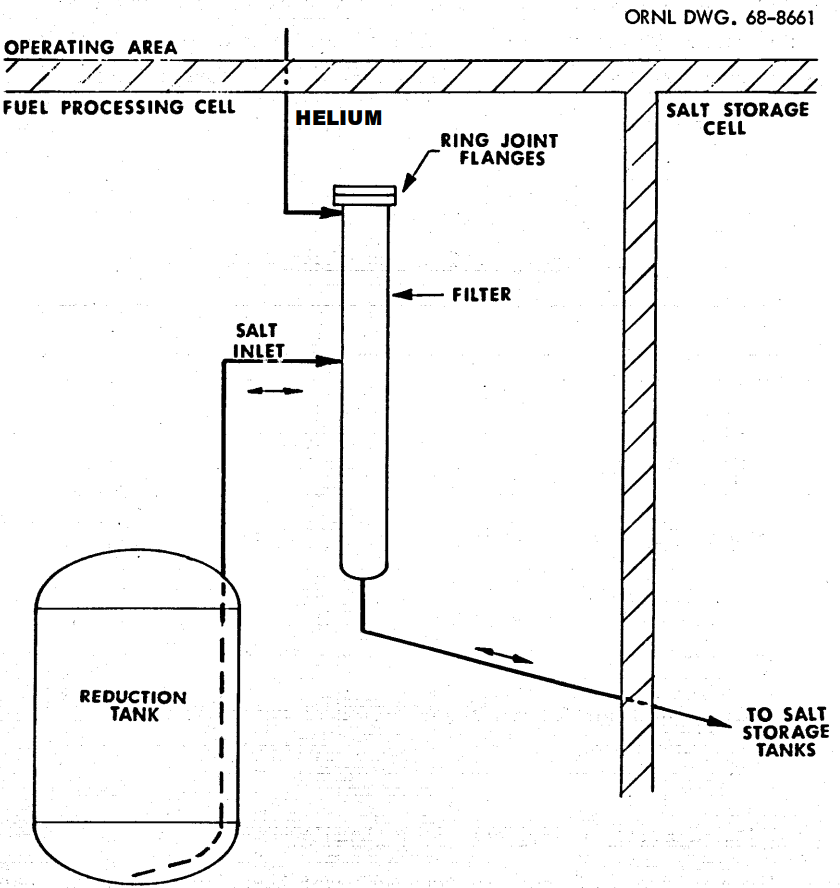
\includegraphics[width=.75\textwidth]{ch2/large_molten_salt_filter_layout.png}
	\caption{Schematic flow diagram of the large molten salt mechanical filter 
		designed and operated during the \gls{MSRE} (figure reproduced from 
		Lindauer \emph{et al.} \cite{lindauer_design_1969}).}
	\label{fig:large_filter_layout}
\end{figure}

In this work, we assumed ideal and constant separation efficiency in the 
filtering system. However, in the future, a physics-driven mathematical 
formula can be used when the experimental data or analytical model will be 
available.


\subsection{Fuel chemical processing facility} \label{sec:chemical_processing}
In addition to noble gases, noble and semi-noble metals, the fuel salt 
reprocessing system must extract other \glspl{FP} such as lanthanides. These 
absorb fewer neutrons than $^{135}$Xe, but their removal is crucial to 
guarantee normal operation. Meanwhile, lanthanides have relatively high 
solubility in the carrier salt and must be removed by chemical extraction. 

In thorium-fueled \gls{MSR} designs, $^{232}$Th in the fuel salt absorbs 
thermal neutrons and produces $^{233}$Pa, which then decays into the fissile 
$^{233}$U (Figure~\ref{fig:th_u_reaction}). Protactinium presents a challenge  
since it has a large absorption cross section in the thermal energy spectrum. 
Accordingly, $^{233}$Pa is continuously removed from the fuel salt into a 
protactinium decay tank to allow $^{233}$Pa to decay to $^{233}$U without 
poisoning the reactor. This feature allows the thorium-fueled \gls{MSR} to 
avoid neutron losses to protactinium, keeps fission products  on a trace 
level, and increases the efficiency of $^{233}$U breeding. 

\begin{figure}[htp!] % replace 't' with 'b' to 
	\centering
	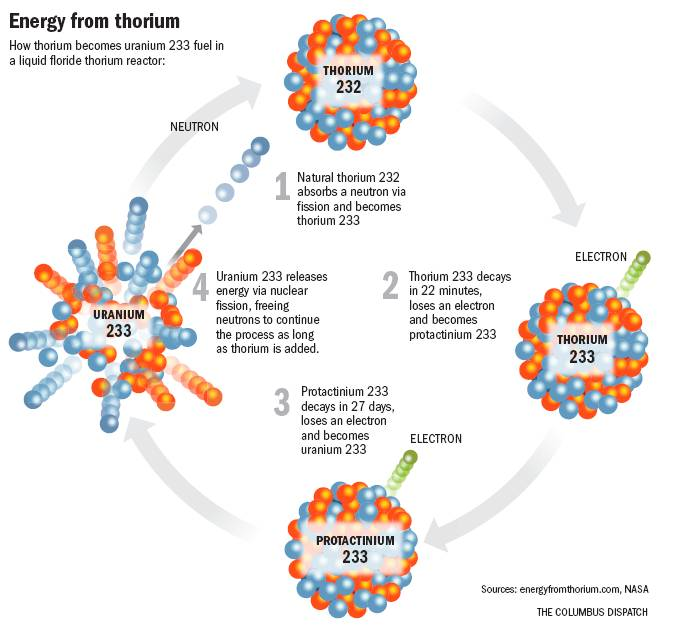
\includegraphics[width=0.57\textwidth]{ch2/th_u_cycle.jpg}
	\caption{Production of $^{233}$U from $^{232}$Th  (reproduced from 
	Sorensen \cite{sorensen_one-fluid_2006}).}
	\label{fig:th_u_reaction}
\end{figure}

Many authors report that a liquid-liquid reductive extraction process is the 
best option for removing protactinium and soluble fission products from 
molten fluoride salts \cite{briggs_molten-salt_1969, delpech_molten_2010, 
	doligez_coupled_2014}. In that process, the protactinium or lanthanides 
	can be 
selectively stripped from the salt into liquid bismuth due to different 
chemical potentials. Moreover, the \gls{MSRE} experience indicated that the 
extraction could be carried out rapidly and continuously  
\cite{whatley_engineering_1970}.

The principal scheme of the \gls{MSBR} reprocessing facility concept is shown 
in Figure~\ref{fig:material_flow}. The fuel salt is first temporarily stored 
for cooling and decay of the shortest-lived fission products, then it is 
directed to the primary fluorinator. There, most of the uranium is removed by 
fluorination to UF$_6$. After that, the salt is routed to an extraction column 
where it is combined with a mixture containing metallic bismuth, lithium, and 
thorium reductants. The remaining uranium and protactinium are reductively 
extracted to a bismuth solution, leaving a salt that only contains fission 
products dissolved in carrier salt (base composition LiF-BeF$_2$-ThF$_4$). The 
salt then goes through a reduction column where UF$_6$ is reduced to UF$_4$,  
preparing it for return to the reactor. BeF$_2$ and ThF$_4$ are also added, 
and all residual bismuth is removed from the salt. After a final cleanup step 
and valence adjustment, the purified salt returns to the reactor 
\cite{carter_design_1972, sorensen_one-fluid_2006}.

\begin{figure}[htp!] % replace 't' with 'b' to 
	\centering
	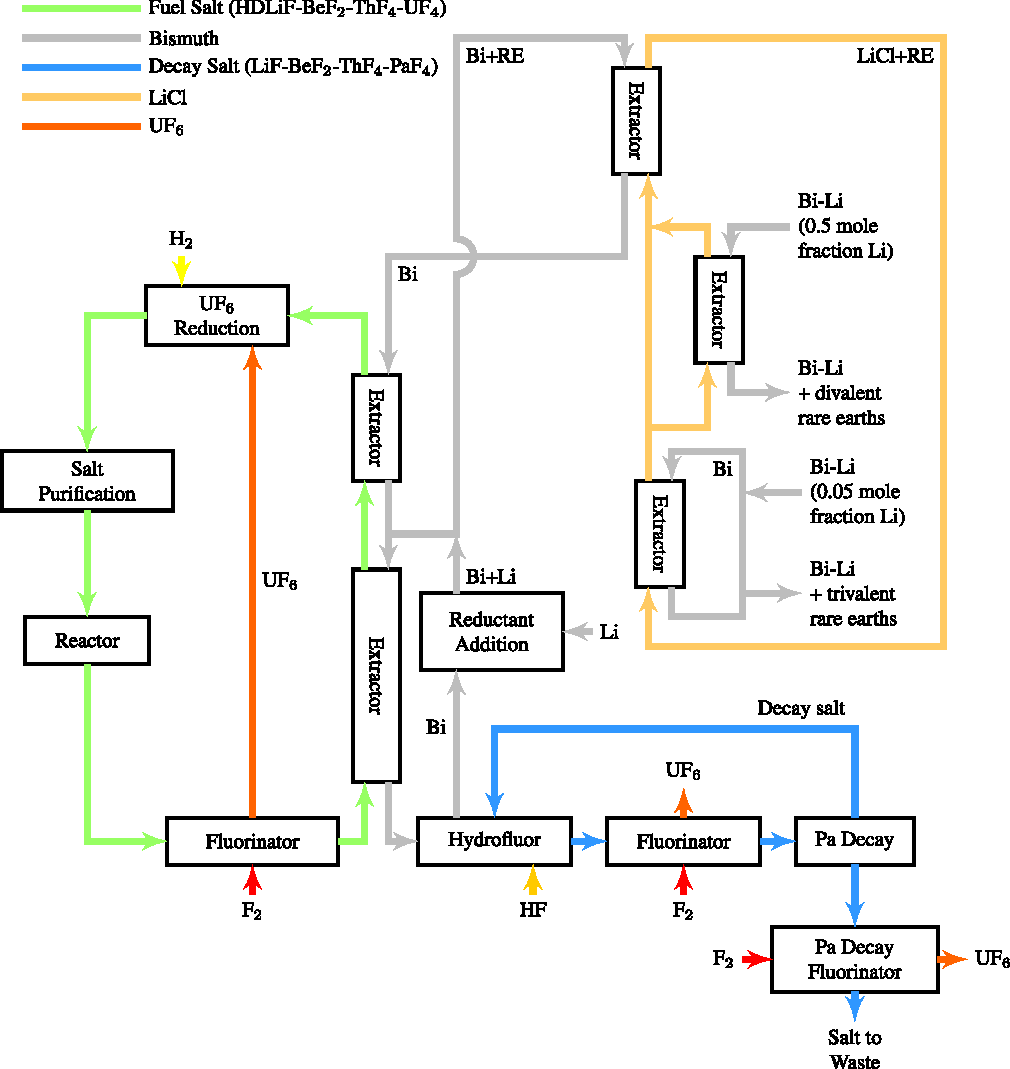
\includegraphics[width=1.01\textwidth]{ch2/flowsheet.pdf}
	\caption{Simplified block diagram of chemical processing scheme for 
		single-fluid \gls{MSBR} (reproduced from Sorensen 
		\cite{sorensen_one-fluid_2006}). \emph{RE} represents the rare 
		earth elements extracted from the salt.}
	\label{fig:material_flow}
\end{figure}

The bismuth accommodating some uranium and protactinium is routed to a 
hydrofluorination column where metallic solutes in the bismuth are oxidized 
into their fluoride forms in the presence of a decay salt\footnote{The decay 
salt contains UF$_4$, PaF$_4$, ThF$_4$ and fission products. Uranium produced 
after $^{233}$Pa decay is extracted and directed back into the reactor. Decay 
salt is the precursor for the waste salt as it was periodically discarded  
every 220 days \cite{robertson_conceptual_1971}.}. The decay salt, containing 
UF$_4$, PaF$_4$, and ThF$_4$, passes into a decay tank where $^{233}$Pa 
decays to $^{233}$U. The uranium generated by protactinium decay is removed 
through fluorination to UF$_6$ and directed to the reduction column to refuel 
the purified fuel salt. A  hydrofluorinator and a fluorinator can remove 
approximately 95\% of the uranium from the stream 
\cite{robertson_conceptual_1971}.

The fully processed salt, on its way back to the reactor, has uranium added 
from the protactinium decay tank at the rate required to maintain or adjust 
the uranium concentration in the reactor (and, consequently, control the 
reactivity). Adding fissile material is performed by sparging the salt with 
UF$_6$ and hydrogen to produce UF$_4$ in the salt and HF gas 
\cite{robertson_conceptual_1971}.

After these separation steps, the fuel salt stream from the protactinium 
isolation system contains only traces of protactinium and uranium but contains 
practically all of the rare earths. A fraction of this salt stream is 
redirected to a reductive extraction process for removing rare earths.  The 
principal scheme of a rare earth removal system is shown in  
Figure~\ref{fig:rare-earth-removal}. A molten salt flow that contains 
rare earth fluorides is fed to the center of an extraction column. The salt 
flows countercurrent to a liquid bismuth stream, which contains thorium and 
lithium. In the upper part of the column, the rare earths are reduced and 
transferred to the downflowing liquid metal stream. Below the feed point, the 
rare earth concentration is increased in the salt and metal streams in order 
to produce a concentration high enough for disposal 
\cite{briggs_molten-salt_1969}.
\begin{figure}[htbp!]
	\centering
	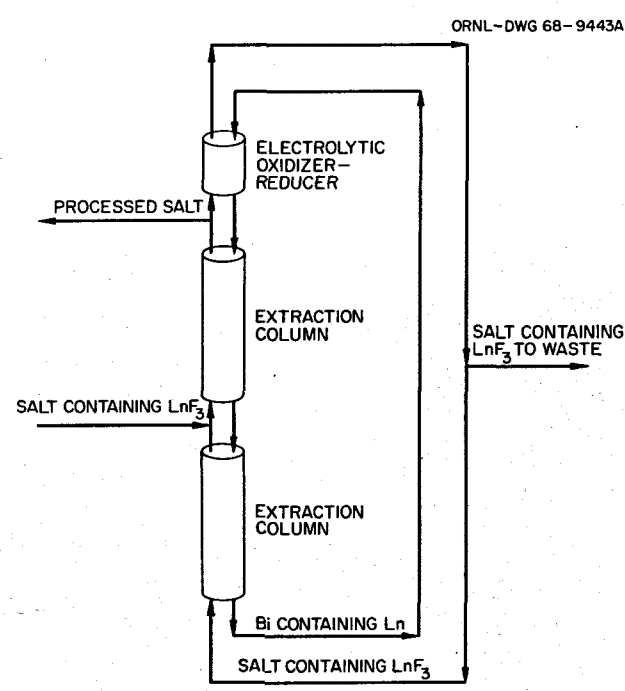
\includegraphics[width=0.45\textwidth]{ch2/rare-earths-removal-system.png}
	\caption{Rare earth removal from a fuel salt by reductive extraction 
		(figure reproduced from Briggs \emph{et al.} 
		\cite{briggs_molten-salt_1969}).}
	\label{fig:rare-earth-removal}
\end{figure}

While it is out of the scope of this work to derive the accurate  
chemistry-based mathematical formula for rare earths and protactinium 
separation efficiency, this work seeks to provide a flexible tool that is able 
to simulate chemical processes in significant detail concerning vital system 
design parameters.

\section{Serpent overview}
Serpent is a continuous-energy Monte Carlo neutronics software capable of 
solving the neutron transport problem by tracking individual neutrons within 
the problem geometry and using the stochastic method to determine the chain of 
events for each neutron \cite{leppanen_serpent_2014}. Serpent is under active 
development at the VTT Technical Research Centre of Finland since 2004, where 
it was initially conceived as a tool to simplify group constant generation in 
a high-fidelity Monte Carlo environment. Serpent is now a widely used  
transport code, used by more than 500 registered individuals in 155 
organizations located in 37 countries around the world. The burnup calculation 
capability in Serpent is based on built-in calculation routines without using 
any external solvers. A restart feature enables fuel shuffling simulation or 
applying any modifications to the input by dividing the calculation into 
several parts, which is crucial for online reprocessing simulations.

The latest version, Serpent 2, supports advanced geometries and has advanced 
burnup capabilities, including online refueling capabilities, which are 
necessary for neutronic computations of pebble-bed reactors and liquid-fueled 
\glspl{MSR} \cite{aufiero_extended_2013}. Unfortunately, built-in online 
refueling features are still under active development, undocumented and the 
discussion forum for Serpent users is the only useful source of information at 
the moment \cite{aufiero_extended_2013}. Additionally, multi-physics 
simulations using Serpent 2 have been demonstrated, including  calculations 
with thermal-hydraulics, \gls{CFD}, and fuel performance codes 
\cite{leppanen_numerical_2015}. 

Serpent 2 can be effectively run in parallel on computer clusters and 
multi-core workstations. Parallelization is handled by thread-based OpenMP, 
which enables all processors to use shared memory space. Calculations can be 
divided into several nodes by distributed-memory \gls{MPI} parallelization. 
Serpent 2  is an improvement upon Serpent 1, and contains a complete redesign 
of memory management using hybrid OpenMP \cite{dagum_openmp_1998} + \gls{MPI} 
parallelization.  This hybrid parallelization is substantial for depletion 
calculations using computer clusters with multiple nodes and allows us to 
achieve significant speed-up in depletion calculations on computer clusters 
with more than 4,000 cores \cite{leppanen_serpent_2014}. 

Simulations herein were performed using Serpent 2 version 2.1.31 on both the 
National Center for Supercomputing Applications' Blue Waters and Idaho 
National Laboratory's Falcon supercomputers. The JEFF-3.1.2 
\cite{oecd/nea_jeff-3.1.2_2014} and ENDF/B-VII.1 
\cite{chadwick_endf/b-vii.1_2011} libraries provided nuclear data 
for all calculations in this dissertation. 

\section{Simulation tool design and capabilities}\label{sec:tool_design}
The first version of the SaltProc tool for calculating \gls{MSR} fuel 
composition evolution, taking into account an online reprocessing system,  
was developed in 2018 as a part of the M.S. thesis  
\cite{rykhlevskii_arfc/saltproc_2018, rykhlevskii_advanced_2018}. The tool was 
designed to expand Serpent 2 depletion capabilities for modeling liquid-fueled 
\glspl{MSR} with online fuel reprocessing system. SaltProc v0.1 uses 
HDF5 
\cite{the_hdf_group_hierarchical_1997} to store data and uses the PyNE Nuclear 
Engineering Toolkit \cite{scopatz_pyne_2012} for Serpent 2 output file parsing 
and nuclide naming. SaltProc v0.1 is an open-source python package that uses a 
batch-wise approach to simulate continuous feeds and removals in \glspl{MSR}. 

SaltProc v0.1 only allows 100\% separation efficiency for either specific 
elements or groups of elements at the end of the specific ``cycle 
time''\footnote{The \gls{MSBR} program defined ``cycle time'' as the time 
required to remove 100\% of a target nuclide from a fuel salt  
\cite{robertson_conceptual_1971}.}. Capabilities of the developed tool, 
working with the Monte Carlo software Serpent 2, were demonstrated using the 
full-core MSBR design for a simplified case with ideal removal efficiency 
(100\% of mass for target elements removed) \cite{rykhlevskii_modeling_2019}. 
The SaltProc v0.1 architecture and the principal structure was not designed 
for flexible implementation of sophisticated online reprocessing systems, 
including realistic variable extraction efficiencies. 

For the current work, SaltProc v0.1 was completely refactored using \gls{OOP} 
to create a comprehensive generic tool to realistically model complex 
\gls{MSR} fuel reprocessing systems while taking into account variable 
extraction efficiencies, time-dependent core geometry, and the mass balance 
between the core and the reprocessing plant.

\subsection{Software architecture} \textbf{This section needs to be updated 
when the structure will be finalized.}

The SaltProc v1.0 python toolkit couples directly with Serpent 2 input 
and output files, to couple the reprocessing system to depletion calculation. 
Python 3 \gls{OOP} standard features are used to create a flexible, 
user-friendly tool with great potential for further improvement and 
collaboration. Figure~\ref{fig:saltproc_class} shows the SaltProc v1.0 class 
structure which includes 4 main classes:
\begin{figure}[ht!] % replace 't' with 'b' to \centering
	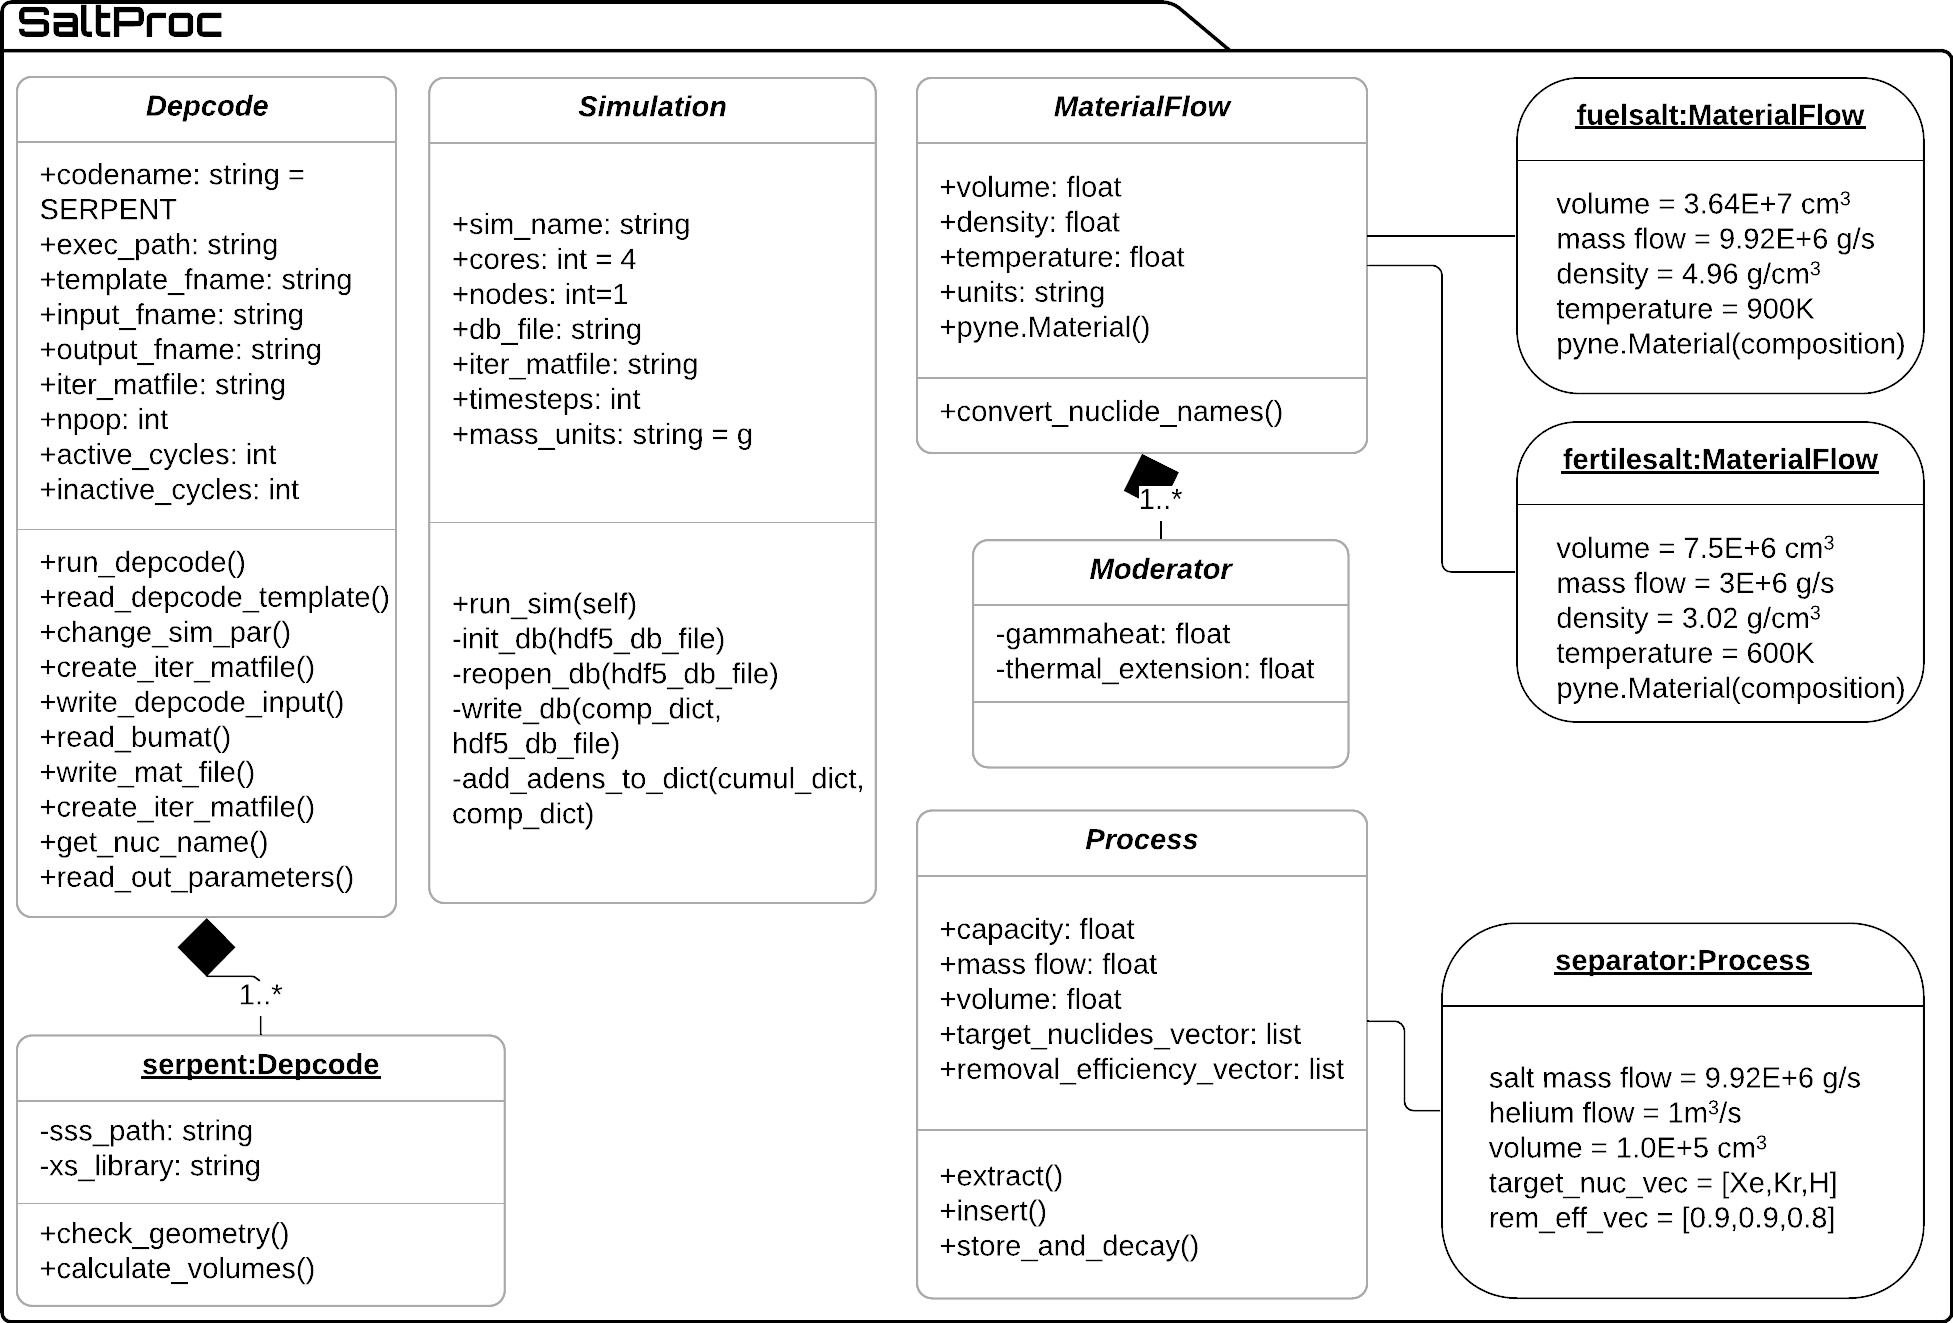
\includegraphics[width=1.01\textwidth]{ch2/saltproc_class_diagram.png}
	\vspace{-0.15in}
	\caption{SaltProc v1.0 python package class diagram in UML 
	notation with examples of object instances.}
	\label{fig:saltproc_class}
\end{figure}
\paragraph{Depcode.}\textit{Depcode} class contains attributes and methods for 
reading the user's input file for the depletion software, initial material 
(e.g., fuel and/or fertile salt) composition, principal parameters for burnup 
simulation (e.g., neutron population and number of cycles for Monte Carlo 
neutron transport), and running the depletion code.
\paragraph{Simulation.}\textit{Simulation} class runs Serpent depletion step, 
creates and writes HDF5 database, tracks time, and converts isotopic 
composition vector nuclide names from Serpent to human-readable format.
\paragraph{MaterialFlow.}Each \textit{MaterialFlow} object represents the 
material flowing between \textit{Process} objects  
(figure~\ref{fig:matflow_obj}). All instances of this class 
contain an isotopic composition vector stored in PyNE Material object, mass 
flow rate, temperature, density, volume, and void fraction. Existing PyNE 
Material capabilities convert the units of the isotopic composition vector 
(e.g., from the atomic density provided by Serpent to a mass fraction or 
absolute mass in desired units) and decay the material (i.e., model the 
\gls{MSBR} protactinium decay tank). The main idea of the 
\textit{MaterialFlow} object is to pass detailed information about the salt 
starting at the \gls{MSR} vessel outlet throughout reprocessing components 
(\textit{Processes}), which modify the \textit{MaterialFlow} object before 
depleting the material in the next Serpent burnup step. 
\begin{figure}[ht!] % replace 't' with 'b' to 
	\centering
	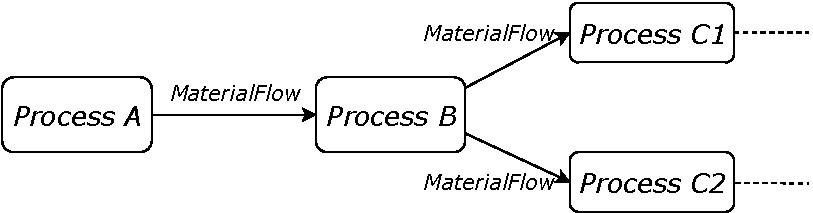
\includegraphics[width=0.7\textwidth]{ch2/materialflow.pdf}
	\vspace{-0.1in}
	\caption{Schematic for passing material data between fuel processing 
		system components.}
	\label{fig:matflow_obj}
\end{figure}
\paragraph{Process.}Each \textit{Process} object represents a 
realistic fuel processing step characterized by its throughput rate, 
volumetric capacity, extraction efficiency for each target element (can be 
a function of many parameters), waste streams, and other process-specific 
parameters. Feed \textit{Process} injects fresh fuel salt 
\textit{MaterialFlow} directly into the reactor core (e.g., adding fissile 
material with a specific mass flow rate to \textit{MaterialFlow} after 
performing all removals).\\


Such a class structure provides outstanding flexibility in simulating 
various \gls{MSR} fuel processing system designs. I created a library of 
various \textit{MaterialFlow} (e.g., fuel salt flow, fertile salt flow, 
refueling salt flow) and \textit{Process} (e.g., helium sparging facility, gas 
separator, nickel filter) objects examples to help a user to create a model of 
a desired reprocessing scheme quickly. At runtime, the user
should connect \textit{Process} objects in series, parallel, or both with 
\textit{MaterialFlow} objects to form a comprehensive reprocessing system. To 
make the reprocessing system definition self-explanatory and straightforward, 
I employed standardized graph description language, \emph{dot}, which is 
widely used in Computer Science \cite{koutsofios_drawing_1996}. The 
reprocessing plant structure described with \emph{dot} can be simply plotted 
using Graphviz \cite{ellson_graphviz_2003}, and those plots can be used for 
analysis, optimization, and publication purposes. The user also had the  
flexibility to create custom objects with desired attributes and methods and 
contribute back to the code package using GitHub  
(https://github.com/arfc/saltproc).	

\subsection{Tool flowchart}
Figure~\ref{fig:saltproc_flow} illustrates the online reprocessing simulation 
algorithm coupling SaltProc v1.0 and Serpent. A \emph{json}-compatible 
user input file for SaltProc contains parameters such as paths to depletion 
software executable, neutron population and number of criticality cycles, 
depletion history, total heating power, and list of files with the core 
geometry definition. To perform a depletion step, SaltProc v1.0 reads a 
user-defined Serpent template file. This file contains input parameters such 
as the path to a nuclear data library, material isotopic composition at 
startup, burnup calculation parameters, and boundary conditions. SaltProc v1.0 
fills in the template file and runs Serpent single-step depletion. 

After the depletion calculation, SaltProc v1.0 reads the depleted fuel 
composition file into the \textit{MaterialFlow} object 
(\textit{core\textunderscore outlet} in figure~\ref{fig:saltproc_flow}). This 
object contains an isotopic composition vector, total volume of material, 
total mass, mass flow rate, density, temperature, void fraction, etc. For the 
simplest reprocessing case, when all fuel processing components are located 
in-line (100\% of total material flow goes through a chain of separation 
components), the \textit{core\textunderscore outlet} object is flowing 
sequentially between \textit{Processes}, and each \textit{Process} is removing 
a mass fraction of target elements with specified extraction efficiency. 
Afterward, the removed material mass is compensated by fresh fuel salt to 
maintain the salt inventory in a primary loop. Finally, resulting isotopic 
composition after reprocessing is stored in the HDF5 database and dumped in a 
new composition file for the next Serpent depletion run. SaltProc v1.0 also 
stores isotopic composition before reprocessing and waste stream from each 
fuel processing component in the HDF5 database. 
\begin{figure}[ht!] % replace 't' with 'b' to \centering
	\centering
	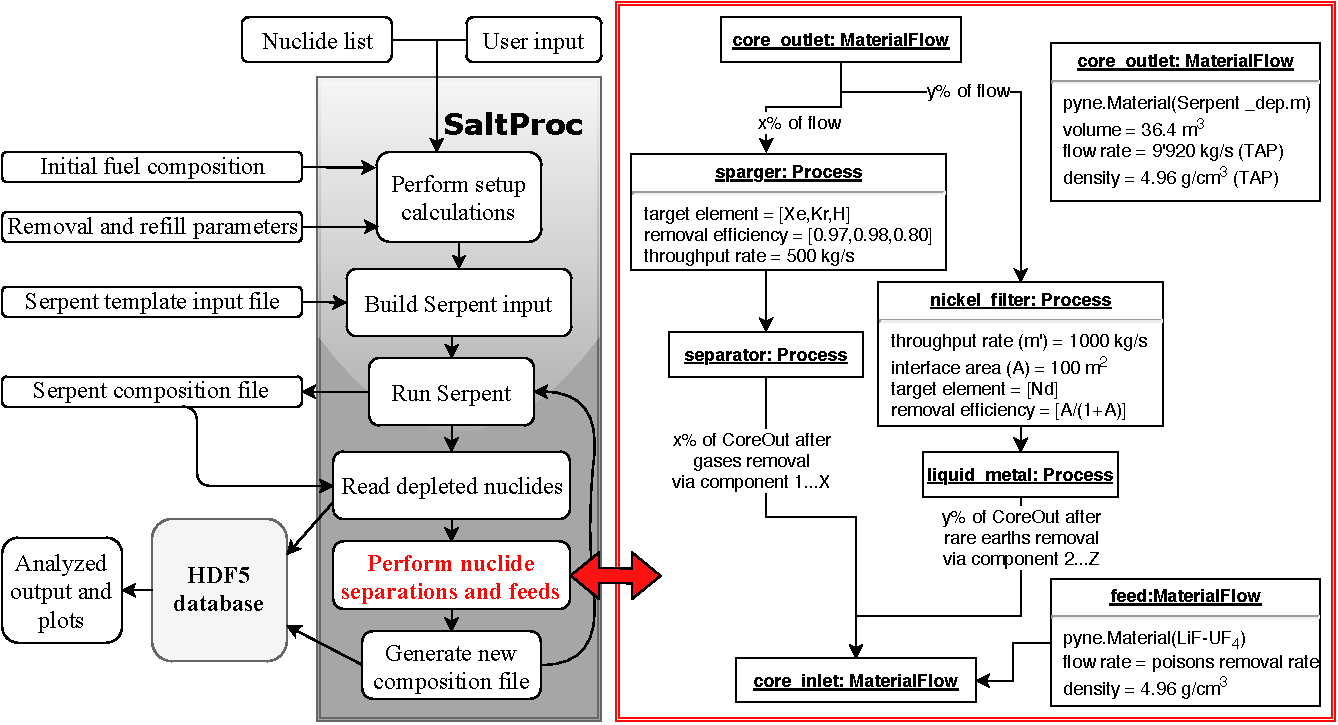
\includegraphics[width=1.01\textwidth]{ch2/saltproc_flowchart.pdf}
	\vspace{-0.15in}
	\caption{Flow chart for SaltProc v1.0 python package.}
	\label{fig:saltproc_flow}
\end{figure}

For a more general case with multiple concurrent extraction processes, a 
separate \textit{MaterialFlow} object is created for each branch with a 
user-defined mass flow rate (e.g., 90\% of total mass flow rate flows via left 
branch and 10\% throughout a right branch). The total mass and isotopic 
composition vector for each \textit{MaterialFlow} object are calculated as a 
fraction of incoming \textit{core\textunderscore outlet} flow. Then each 
\textit{MaterialFlow} object is passed via a cascade of \textit{Processes} to 
separate selected chemical elements with specific efficiency. Finally, the 
left-hand-side branch \textit{MaterialFlow} object is merged with the 
right-hand-side, and similarly to the previous case, fresh fuel salt feed 
compensates the loss of mass in separation facilities and keeps fuel salt mass 
in a primary loop constant.

The class diagram (figure~\ref{fig:saltproc_class}) allowing to model the 
operation of a complex, multi-zone, multi-fluid \gls{MSR} and is sufficiently 
general to represent myriad reactor systems. SaltProc v1.0 only stores and 
changes the isotopic composition of the fuel stream, which makes it a flexible 
tool to model any geometry: an infinite medium, a unit cell, a multi-zone 
simplified assembly, or a full-core. This flexibility allows the user to 
perform simulations of varying fidelity and computational intensity. 
SaltProc v1.0 is an open-source tool (but a user needs Serpent 2.1.31 
installed to use SaltProc v1.0), available on GitHub. It leverages unit and 
continuous tests crucial for sustainable development \cite{krekel_pytest_2004, 
travis_travis-ci/travis-api_2016}. The documentation is automatically 
generated using Sphinx \cite{brandl_sphinx_2009} and can be found here: 
\emph{https://arfc.github.io/saltproc/}. In summary, the development approach 
of SaltProc v1.0 is focused on producing a generic, flexible and expandable 
tool to give the Serpent 2 Monte Carlo code the ability to conduct advanced 
in-reactor fuel cycle analysis as well as simulate many online refueling and 
fuel reprocessing systems.

\subsection{Reactivity control module}
Simulation of specific \gls{MSR} concepts requires to change the reactor core 
geometry during lifetime-long operation modeling. For instance, the \gls{TAP} 
concept aims to increase the core lifetime by using continuous fresh fuel 
feeds, removal of \glspl{FP}, and configurable moderator rod assemblies to 
compensate for negative reactivity insertion due to fissile material burnup. 
The concept proposes to maintaining reactivity in the long term by replacing 
stationary moderator assemblies with more highly populated lattices to 
increase the moderator-to-fuel ratio \cite{betzler_assessment_2017-1}. 
SaltProc v1.0 can switch from one file containing the core geometry to 
another core geometry (e.g., with larger moderator-to-fuel ratio) if effective 
multiplication factor, $k_{eff}$, falls below a specific limit (e.g., 1.002). 
This unique capability allows SaltProc v1.0 to analyze the fuel cycle 
performance of any liquid-fueled \gls{MSR} system, including advanced designs 
with a moving moderator.

%\section{Multi-component fuel salt reprocessing system}
\section{Concluding remarks}
In this chapter, the overview of the fuel salt reprocessing plant has first 
been presented. I described various components of the plant and the physical 
or chemical mechanism responsible for neutron poisons extraction from the 
salt. General core physics aspects and Serpent 2 depletion software 
capabilities have then been discussed. I also introduced SaltProc, Python 
package, developed and used to simulate continuous feeds and removals in 
various \gls{MSR} designs.

In the following chapters, SaltProc v1.0 will be demonstrated and validated 
for two liquid-fueled \gls{MSR} designs.